\section{Parquet} \label{sec:parquet}

The first thing to understand about parquet is that it is a \textit{File Storage Format}.
As such, it is best thought of as an alternative to JSON or CSV.
While they are not its main competitors, most readers will be familiar with them so we will use them as easy comparisons.
As a file storage format, Parquet is designed to be language-agnostic.

This section will focus on the two core components of Parquet, columnar storage and how Parquet stores nested objects.

\subsection{Row storage versus columnar storage}

We assume the reader is familiar with the basic tradeoffs associated with row storage versus columnar storage.
Thus, we will only briefly recap the differences.

Consider the following table in Figure \ref{fig:table}. \\
\begin{figure}[h]
\centering
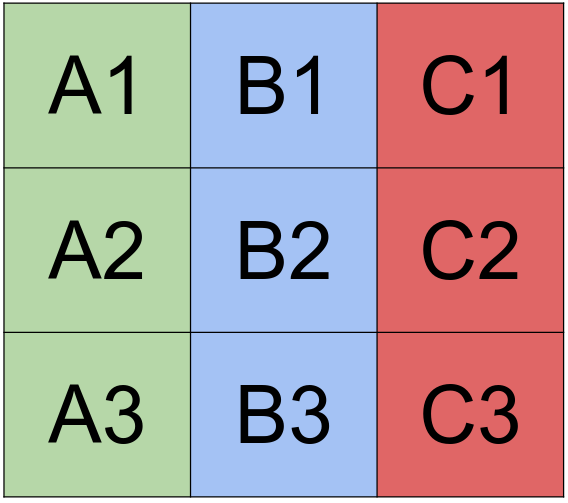
\includegraphics[width=0.3\textwidth]{table.png}
\caption{Example Table with Columns A, B, and C}
\label{fig:table}
\end{figure}

In traditional Row-based DBMS such as PostgreSQL\footnote{https://www.postgresql.org/}, the data is organized in storage one row at a time.
A visual representation is shown in Figure \ref{fig:row-major}. \\
\begin{figure}[h]
\centering
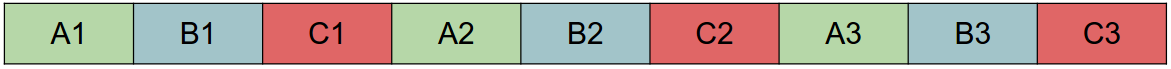
\includegraphics[width=0.8\textwidth]{row-major.png}
\caption{Row-major Storage Layout}
\label{fig:row-major}
\end{figure}

Columnar-based storage formats such as Parquet organize the data such that columns are stored together.
The Table from Figure \ref{fig:table} would thus be organized in storage as shown in Figure \ref{fig:column-major}.
\begin{figure}[h]
\centering
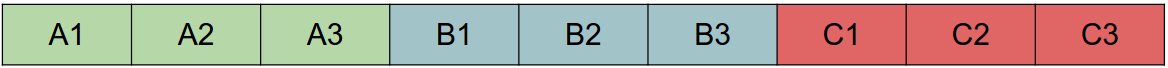
\includegraphics[width=0.8\textwidth]{column-major.png}
\caption{column-major Storage Layout}
\label{fig:column-major}
\end{figure}
\\

This has three major advantadges \cite{dremel-parquet:Twitter}:
\begin{description}
\item[Compression] Data in a column is more homogenous which allows for better compression. Our Benchmark results in Section \ref{sec:results} confirm this.
\item[I/O] For column-based queries such as $max$ or $avg$, only the relevant subset of data needs to be scanned.
\item[Processor Encoding] Data in the same Column has the same type which means optimized storage engines can use encodings better suited for modern processors
\end{description}

\subsection{Nested Objects}
\label{section:parquet-nested}
To store nested objects, Parquet needs a schema.
The schema used for Parquet is very similar to the one used by Protobuf\footnote{https://developers.google.com/protocol-buffers/}.
A field thus is one of three possibilities

\begin{description}
\item[required] The field exists once and only once
\item[optional] The field exists once or zero times
\item[repeated] The field exists zero ore more times
\end{description}

Or formally, the schema is defined as:
\begin{equation}
\tau = \mathbf{dom} \,|\, \langle A_{1} : \tau [*|?], \, \dots \,, \,  A_{n} : \tau [*|?]\rangle
\end{equation}
Where $\tau$ is an atomic type or record type \cite{dremel:melnik}. Atomic types are strings or integers, for example.
$*$ indicates that a field is repeated and $?$ indicates that it is optional.

To give a concrete example, TODOOOOOOOOOOoOooooOOOOoooooOOOOOO  //TODO